\documentclass{a4beamer}
%% Lectures - common definitions

\usextensions{tikz}
\usetikzlibrary{shapes.multipart,shapes.callouts,shapes.geometric}
\input{fix-callouts.inc} % Fixes absolute positioning of rectangle callouts

\newif\ifbigpages \bigpagesfalse
\ifdim\paperwidth >20cm
	\bigpagestrue
\fi

\tikzset{%
	note/.style={rectangle callout,draw=none,callout pointer width=1em,%
		align=flush left,font=\footnotesize,inner sep=0.5em,%
		fill=blue!15,fill opacity=0.95,text opacity=1.0,callout absolute pointer=#1},
	node distance=2em and 2.75em
}
\ifbigpages
	% Scale all arrow tips by the factor of 2.5
	\let\old@pgf@arrow@call=\pgf@arrow@call
	\def\pgf@arrow@call#1{%
		\@tempdima=\pgflinewidth%
		\pgfsetlinewidth{2.5\pgflinewidth}%
		\old@pgf@arrow@call{#1}%
		\pgfsetlinewidth{\@tempdima}%
	}
	\def\pgfarrowsleftextend#1{\pgfmathsetlength{\pgf@xa}{1.5*#1}}
	\def\pgfarrowsrightextend#1{\pgfmathsetlength{\pgf@xb}{1.5*#1}}
\fi

%% Load listings package
\usepackage{listings}

%% Are we inside a comment?
\newif\iflstcomment \lstcommentfalse

\lstset{%
	tabsize=4,
	showstringspaces=false,
	basicstyle=\linespread{1.25}\ttfamily\small,
	keywordstyle=\bfseries,
	commentstyle=\lstcommentstyle,
	numbers=left,
	numberstyle=\footnotesize\color{gray},
	xleftmargin=2.5em,
	extendedchars=true,
	escapechar=\$,
	escapebegin=\iflstcomment\begingroup\lstcommentstyle\fi,
	escapeend=\iflstcomment\endgroup\fi
}

\def\lstcommentstyle{\color{gray}}

\lst@AddToHook{AfterBeginComment}{\global\lstcommenttrue}
\let\orig@lst@EndComment=\lst@EndComment
\def\lst@EndComment{\global\lstcommentfalse\orig@lst@EndComment}
\lst@AddToHookAtTop{EOL}{%
	\lst@ifLmode\global\lstcommentfalse\fi% XXX Sloppy way to determine comment end
}

%% Python with docstrings treated as comments
\lstdefinelanguage[doc]{python}[]{python}{%
	deletestring=[s]{"""}{"""},%
	morecomment=[s]{"""}{"""}%
}%

%% JavaScript language
\lstdefinelanguage{javascript}%
	{morekeywords={break,case,catch,%
		const,constructor,continue,default,do,else,false,%
		finally,for,function,if,in,instanceof,%
		new,null,prototype,%
		return,switch,this,throw,%
		true,try,typeof,var,while},%
	sensitive,%
	morecomment=[l]//,%
	morecomment=[s]{/*}{*/},%
	morestring=[b]",%
	morestring=[b]',%
}[keywords,comments,strings]%

%% C# language (4.0?)
\lstdefinelanguage{csharp}%
	{morekeywords={abstract,as,%
		base,bool,byte,case,catch,char,%
		checked,class,const,continue,%
		decimal,default,delegate,do,double,%
		else,enum,event,explicit,extern,%
		false,finally,fixed,float,for,foreach,%
		goto,if,implicit,in,int,interface,%
		internal,is,lock,long,%
		namespace,new,null,object,operator,out,%
		override,params,private,protected,public,%
		readonly,ref,return,sbyte,sealed,%
		short,sizeof,stackalloc,static,string,%
		struct,switch,this,throw,true,try,%
		typeof,uint,ulong,unchecked,unsafe,ushort,%
		using,virtual,void,volatile,while%
	},%
	sensitive,%
	morecomment=[l]//,%
	morecomment=[s]{/*}{*/},%
	morestring=[b]",%
	morestring=[b]',%
}[keywords,comments,strings]%

%% Translation for fact environment
\deftranslation[to=russian]{Fact}{Наблюдение}

%% Inline code snippets
\def\code#1{\texttt{#1}}
\def\codekw#1{\code{\textbf{#1}}}

\def\quoteauthor#1{\par\footnotesize\upshape\hfill—~#1}

%% English term
\def\engterm#1{(англ. \textit{#1})}
%% Term with explanation below (to be used in diagrams)
\def\termwithexpl#1#2{#1\strut{}\\\small\color{gray}(\textit{#2})\strut{}}
%% External link
\def\extlink#1#2{\href{#1}{\color[rgb]{0.7,0.7,1.0}\dashbar{#2}}}
%% Internal link
\def\inlink#1#2{\hyperlink{#1}{\color[rgb]{0.7,0.7,1.0}\dashbar{#2}}}
%% Explanation for a list item
\def\itemexpl#1{\begingroup\small\vspace{0.75ex}#1\par\endgroup}



\usetikzlibrary{shapes.misc}
\usepackage{multicol}


\lecturetitle{Программная инженерия. Лекция №13 — Тестирование}
\title[Тестирование]{Тестирование программного обеспечения}
\author{Алексей Островский}
\institute{\small{Физико-технический учебно-научный центр НАН Украины}\vspace{2ex}}
\date{05 марта 2015 г.}

\begin{document}
	\frame{\titlepage}

	\section{Введение}

	\subsection{Основные понятия}

	\frame{
		\frametitle{Основные понятия тестирования}

		\textbf{Этапы возникновения сбоев} в программе:
		\begin{enumerate}
			\item
			программист совершает \emph{ошибку} (error, mistake);
			\item
			ошибка приводит к \emph{дефекту} (defect, fault, bug) в исходном коде;
			\item
			при определенных условиях исполнения дефект приводит к \emph{сбою программы} (program failure).
		\end{enumerate}

		\vspace{1ex}
		\textbf{Тест} — набор входных данных и прочих условий (напр., характеристики операционной системы и оборудования),
		которые полностью определяют ход выполнения программы.

		\vspace{1ex}
		\textbf{Цель тестирования} — локализация и устранение дефектов, соответствующие всем~сбоям программы,
		обнаруженным с~помощью~тестов.

		\vspace{2ex}
		\begin{tikz*}[every node/.style={rectangle,align=center}]
			\node (all) at (0, 0) {
				Прогон \emph{всех} тестов невозможен \\
				даже для простых систем.
			};
			\node[right=of all] (imply) {
				\Large $\Rightarrow$
			};
			\node[right=of imply] (info) {
				Необходим отбор \\
				\emph{информативных} тестов.
			};
		\end{tikz*}
	}

	\subsection{Определение тестирования}

	\frame{
		\frametitle{Тестирование ПО}

		\begin{Definition}
			\textbf{Тестирование ПО} — это процесс проверки готовой программы в~\emph{статике} (обзоры кода, инспекции и~т.\,п.)
			и~\emph{динамике} (прогон программы на~тестовых данных) с~целью обеспечить ее~соответствие заданным требованиям.
		\end{Definition}

		\vspace{1ex}
		\textbf{Режимы тестирования:}

		\begin{center}\small
			\begin{tabular}{|l|p{0.35\textwidth}|p{0.35\textwidth}|}
				\hline
				& Валидация & Обнаружение дефектов \cr
				\hline
				Цели & \raggedright демонстрация разработчикам и~заказчикам
					соответствия программного продукта требованиям &
					\raggedright определение границ применимости ПО; поиск ситуаций,
					в которых поведение некорректно, нежелательно или не удовлетворяет спецификации. \cr
				\hline
				Содержание &
					\raggedright ожидаемые сценарии использования ПО &
					\raggedright экстремальные сценарии использования. \cr
				\hline
				Выбор тестов &
					\raggedright исходя из спецификации системных требований &
					\raggedright для отработки исключительных ситуаций. \cr
				\hline
			\end{tabular}
		\end{center}
	}

	\subsection{Виды тестирования}

	\frame{
		\frametitle{Виды тестирования}

		\textbf{По объекту тестирования:}
		\begin{itemize}
			\item
			статические методы (процессы верификации и валидации — следующая лекция);
			\item
			динамические методы.
		\end{itemize}

		\vspace{1ex}
		\textbf{С точки зрения при составлении тестов:}
		\begin{itemize}
			\item
			\textbf{Белый ящик} \engterm{white box testing}, структурное тестирование
			— тестирование внутренних структур и операций ПО.

			\item
			\textbf{Черный ящик} \engterm{black box testing} — тестирование функциональности, доступной конечному пользователю ПО.

			\item
			\textbf{Серый ящик} \engterm{gray box testing} — тестирование ПО с~частичным знанием о~его~внутренней структуре.
		\end{itemize}
	}

	\subsection{Место в разработке}

	\frame{
		\frametitle{Место тестирования в разработке ПО}

		\begin{figure}
			\begin{tikz*}[%
	every node/.style={rectangle,align=center,minimum height=2.25em}
]
	\node(req) [draw] {Инженерия требований};
	\node(req-doc) [right=5em of req] {Спецификация требований};
	\node(design) [below right=2em and -3em of req,draw] {Проектирование};
	\node(arch) [right=4em of design] {Архитектура};
	\node(impl) [below right=2em and -3em of design,draw] {Имплементация};
	\node(sw) [right=4em of impl] {Программный продукт};
	\node(test) [below right=2em and -3em of impl,draw] {\alert{Тестирование}};
	\node(maint) [below right=2em and -3em of test,draw] {Сопровождение};
	
	\draw[->] (req) to (design);
	\draw[->,dashed] (req) to (req-doc);
	\draw[->] (design) to (impl);
	\draw[->,dashed] (design) to (arch);
	\draw[->] (impl) to (test);
	\draw[->,dashed] (impl) to (sw);
	\draw[->] (test) to (maint);
	\draw[->,dotted] (maint) -| (req);
\end{tikz*}

			\caption{В каскадной модели тестирование — отдельный этап разработки, следующий за написанием кода.}
		\end{figure}
	}

	\frame{
		\frametitle{Место тестирования в разработке ПО}

		\begin{figure}
			\begin{tikz*}[%
	node distance=2.0em and 3.0em,
	every node/.style={rectangle,draw,align=center,minimum height=2.5em}
]
	\node(init) {Начальные \\ требования};
	\node(proto) [below=of init] {Разработка \\ прототипа};
	\node(req) [right=of proto] {Конкретизация \\ требований};
	\node(testing) [ellipse,right=of req] {\alert{Тестирование}};
	\node(diff) [below=of $(proto.south)!0.5!(req.south)$] {Внесение \\ изменений};
	\node(release) [below=of diff] {Выпуск};
	\node(customer) [above=of req,ellipse] {Заказчик};
	
	\draw[dashed] (req) to (testing);
	\draw[->] (init) to (proto);
	\draw[->] (proto) to (req);
	\draw[->] (req) to (diff);
	\draw[->] (diff) to (proto);
	\draw[->] (diff) to (release);
	\draw[<->,dashed] (init) to (customer);
	\draw[<->,dashed] (req) to (customer);
\end{tikz*}

			\caption{Согласно эволюционной модели разработки ПО, тестирование неразрывно связано с конструированием.}
		\end{figure}
	}

	\frame{
		\frametitle{Процесс тестирования}

		\begin{enumerate}
			\item
			\textbf{Разработка} тестовых примеров \engterm{test cases}.

			\vspace{0.5ex}
			\textbf{Результаты:} набор тестовых примеров.

			\vspace{0.5ex}
			\item
			\textbf{Подготовка} тестовых данных.

			\vspace{0.5ex}
			\textbf{Результаты:} данные для тестовых примеров.

			\vspace{0.5ex}
			\item
			\textbf{Выполнение программы} на тестовых данных.

			\vspace{0.5ex}
			\textbf{Результаты:} продукты выполнения программы.

			\vspace{0.5ex}
			\item
			\textbf{Сравнение результатов} с ожидаемыми.

			\vspace{0.5ex}
			\textbf{Результаты:} отчеты о тестировании.
		\end{enumerate}

		\vspace{1ex}
		Выполнение тестов и подготовка отчетов может быть \emph{автоматизированным}.
	}

	\frame{
		\frametitle{Фазы тестирования}

		\begin{center}\small
			\begin{tabular}{|l|p{0.275\textwidth}|p{0.3\textwidth}|p{0.225\textwidth}|}
				\hline
				№ & Название & Цель & Ответственные \cr
				\hline
				1 & \raggedright Тестирование при~разработке (\emph{development testing})
					& \raggedright обнаружение дефектов & разработчики \cr
				\hline
				2 & \raggedright Тестирование выпусков (\emph{release testing})
					& \raggedright проверка на соответствие требованиям заказчика
					& \raggedright отдел тестирования \cr
				\hline
				3 & \raggedright Пользовательское тестирование (\emph{user testing})
					& \raggedright выполнение в среде пользователя; уточнение требований.
					& \raggedright пользователи; отдел маркетинга \cr
				\hline
			\end{tabular}
		\end{center}
	}

	\section{При разработке}

	\frame{
		\frametitle{Тестирование при разработке}

		\begin{Definition}
			\textbf{Тестирование при разработке} \engterm{development testing} — совокупность всех видов тестирования,
			осуществляемых непосредственными разработчиками программного продукта.
		\end{Definition}

		\vspace{1ex}
		\textbf{Уровни тестирования:}
		\begin{enumerate}
			\item
			модульное тестирование \engterm{unit testing} — проверка функциональности отдельных методов или классов;
			\item
			компонентное тестирование \engterm{component testing} — проверка программных интерфейсов составных компонентов;
			\item
			системное тестирование \engterm{system testing} — проверка системы в целом;
			тестирование взаимодействий между компонентами.
		\end{enumerate}
	}

	\subsection{Модульное тестирование}

	\frame{
		\frametitle{Модульное тестирование}

		\textbf{Цель:}
		\begin{itemize}
			\item
			проверка методов класса, реализующих отдельные системные требования, с~различными входными данными;
			\item
			тестирование состояний, в~которых может~находиться объект.
		\end{itemize}

		\vspace{1ex}
		\textbf{Этапы модульного теста}
		\begin{enumerate}
			\item
			\textbf{подготовка:} инициализация системы, входных и ожидаемых выходных данных;
			\item
			\textbf{вызов} тестируемых методов или объектов;
			\item
			\textbf{сравнение} результатов вызова с ожидаемым.
		\end{enumerate}

		\vspace{1ex}
		\textbf{Инструменты:}
		\begin{itemize}
			\item
			автоматизированные системы тестирования (xUnit);
			\item
			mock-объекты (упрощенные объекты, реализующие требуемые интерфейсы, напр., БД).
		\end{itemize}
	}

	\frame{
		\frametitle{Подбор модульных тестов}

		\begin{itemize}
			\item
			\textbf{Анализ граничных значений} \engterm{boundary-value analysis}.

			\vspace{0.5ex}
			\begin{figure}
				\begin{tabular}{*{2}{c}c|*{4}{c}c|*{2}{c}c}
	$\cdots$ & -2 & \alert{-1} & \alert{0} & 1 & $\cdots$ & 99 & \alert{100} & \alert{101} & 102 & $\cdots$ \cr
	\hline
	\multicolumn{3}{c|}{некорректно} & \multicolumn{5}{c|}{корректно} & \multicolumn{3}{c}{некорректно}
\end{tabular}

				\caption{Граничные значнения для целочисленной величины, обозначающей процент.}
			\end{figure}

			\vspace{1ex}
			\item
			\textbf{Комбинаторные методы:}
			\begin{itemize}
				\item \extlink{http://en.wikipedia.org/wiki/All-pairs_testing}{уникальные пары значений};
				\item \extlink{http://en.wikipedia.org/wiki/Orthogonal_array_testing}{ортогональные массивы}.
			\end{itemize}

			\vspace{1ex}
			\item
			Выбор на основе \textbf{математической модели} тестируемой системы.

			\vspace{1ex}
			\item
			\textbf{Эвристический подход} — тестирование тех наборов данных, где~легче~всего допустить ошибку.
		\end{itemize}
	}

	\frame{
		\frametitle{Пример — тестирование чисел Фибоначчи (Java / JUnit)}

		\lstinputlisting[language=java]{code-junit.java}
	}

	\subsection{Тестирование компонентов}

	\frame{
		\frametitle{Тестирование компонентов}

		Тестирование компонентов $\simeq$ проверка корректности их интерфейсов.

		\vspace{1ex}
		\textbf{Виды ошибок, связанных с интерфейсами:}
		\begin{itemize}
			\item
			Неправильное использование \engterm{interface misuse}.

			\vspace{0.5ex}
			\textbf{Пример:} параметры некорректного типа или в неправильном порядке при вызове методов.

			\item
			Заблуждения об интерфейсе \engterm{interface misunderstanding}.

			\vspace{0.5ex}
			\textbf{Пример:} бинарный поиск в несортированном массиве.

			\item
			Ошибки синхронизации \engterm{timing errors}.

			\vspace{0.5ex}
			\textbf{Пример:} работа с разделяемой памятью или очередями сообщений
			с различной скоростью обработки данных разными компонентами.
		\end{itemize}
	}

	\frame{
		\frametitle{Подбор тестов компонентов}

		\begin{itemize}
			\item
			Проверка \textbf{граничных значений} параметров методов при работе с внешними компонентами;

			\item
			корректность работы \textbf{с нулевыми указателями} (\textbf{null}) при передаче объектов;

			\item
			возникновение и обработка \textbf{исключительных ситуаций} для~проверки правильного понимания спецификаций;

			\item
			\textbf{стрессовое тестирование} для систем обмена сообщениями;

			\item
			\textbf{варьирование очередности вызовов} при использовании разделяемой памяти.
		\end{itemize}

		\vspace{1ex}
		\textbf{Инструменты:} статические анализаторы кода.
	}

	\subsection{Системное тестирование}

	\frame{
		\frametitle{Системное тестирование}

		\begin{Definition}
			\textbf{Системное тестирование} —
			\begin{itemize}
				\item
				проверка корректности взаимодействия между компонентами программной системы;
				\item
				проверка отсутствия нежелательных побочных эффектов, связанных с~выполнением в~единой среде.
			\end{itemize}
		\end{Definition}

		\vspace{1ex}
		\textbf{Подбор тестов:}
		\begin{itemize}
			\item
			покрытие кода (каждая инструкция должна выполняться $\geq$1 раз);
			\item
			тестирование пользовательского ввода с корректными и некорректными данными;
			\item
			тестирование вариантов взаимодействия с системой;
			\item
			тестирование ожидаемых комбинаций методов.
		\end{itemize}
	}

	\subsection{Разработка через тестирование}

	\frame{
		\frametitle{Разработка через тестирование}

		\begin{Definition}
			\textbf{Разработка через тестирование} \engterm{test-driven development, TDD} — модель разработки ПО,
			основанная на~использовании автоматизированных тестовых вариантов для~определения новой или усовершенствованной функциональности.
		\end{Definition}

		\vspace{1ex}
		\textbf{Область применения TDD:}
		\begin{itemize}
			\item гибкая методология разработки;
			\item экстремальное программирование.
		\end{itemize}

		\vspace{1ex}
		\textbf{Инструменты:} автоматизированные системы тестирования (напр., xUnit).
	}

	\frame{
		\frametitle{Процесс разработки в TDD}

		\begin{center}
			\begin{tikz*}[%
	every node/.style={align=center},
	action/.style={rounded rectangle,draw,minimum height=2.25em,minimum width=10em},
	decision/.style={diamond,draw,minimum width=1em,minimum height=1em},
	label/.style={font=\footnotesize}
]
	\node(func) [action] {Выделение \\ функциональности};
	\node(new-test) [action,below=of func] {Написание теста};
	\node(test) [action,below=of new-test] {Проверка теста};
	
	\node(decision-test) [decision,right=of test] {};
	\node(impl) [action,right=5em of decision-test] {Реализация};
	\node(reg) [action,below=of impl] {Регрессионное \\ тестирование};
	\node(decision-reg) [decision,right=5em of reg] {};
	\node(refactor) [action,below=3.5em of decision-reg] {Рефакторинг};

	\draw[->] (func) -- (new-test);
	\draw[->] (new-test) -- (test);
	\draw[->] (test) -- (decision-test);
	\draw[->] (decision-test) -- node[below,label]{[ошибка]} (impl);
	\draw[->] (decision-test) |- node[right,label,pos=0.25]{[успех]} (new-test);
	\draw[->] (impl) -- (reg);
	\draw[->] (reg) -- (decision-reg);
	\draw[->] (decision-reg) -- node[left,label]{[успех]} (refactor);
	\draw[->] (decision-reg) |- node[right,label,pos=0.25]{[ошибка]} (impl);

	\node(_tmp) [coordinate,left=1.5em of func.west] {};
	\draw[dotted] (refactor) -| (_tmp) [->] -- (func.west);
\end{tikz*}

		\end{center}
	}

	\frame{
		\frametitle{Преимущества TDD}

		\begin{itemize}
			\item
			\textbf{Скрупулезное тестирование} всего выполняемого кода;
			обнаружение дефектов на~ранних стадиях разработки.

			\vspace{0.5ex}
			\item
			\textbf{Автоматизация} регрессионного тестирования.

			\vspace{0.5ex}
			\item
			Упрощение процесса \textbf{отладки и локализации ошибок}.

			\vspace{0.5ex}
			\item
			Повышение \textbf{модульности и гибкости} кода; четкое определение интерфейсов.

			\vspace{0.5ex}
			\item
			Тесты как \textbf{форма документации} программной системы.
		\end{itemize}
	}

	\frame{
		\frametitle{Недостатки TDD}

		\begin{itemize}
			\item
			Невозможность применения для тестирования слабо формализованных
			(пользовательский интерфейс) или комплексных (работа с БД) требований.

			\item
			Ангажированность при написании тестов:
			тесты могут не покрывать возможные сценарии использования из-за неверной трактовки разработчиком
			требований к~системе.

			\item
			Необходимость тщательного планирования разработки
			(тестам должно уделяться адекватное количество времени).

			\item
			Проблема тестирования скрытых (\textbf{private}) полей / методов.
		\end{itemize}
	}

	\section{После разработки}

	\subsection{Тестирование выпусков}

	\frame{
		\frametitle{Тестирование выпусков}

		\begin{Definition}
			\textbf{Тестирование выпусков} \engterm{release testing} — проверка определенного выпуска программного продукта,
			предназначенного для использования вне отдела разработки.
		\end{Definition}

		\vspace{1ex}
		\textbf{Отличия от системного тестирования на этапе разработки:}
		\begin{center}\small
			\begin{tabular}{|p{0.25\textwidth}|p{0.275\textwidth}|p{0.275\textwidth}|}
				\hline
				& Системное тестирование & Тестирование выпуска \cr
				\hline
				\raggedright Ответственные за~тестирование & разработчики & \raggedright независимый отдел тестирования \cr
				\hline
				Цель тестирования & \raggedright определение и исправление ошибок & \raggedright проверка соответствия требованиям \cr
				\hline
				Методы тестирования & «белый ящик» & «черный ящик» \cr
				\hline
			\end{tabular}
		\end{center}
	}

	\frame{
		\frametitle{Виды тестирования выпусков}

		\begin{itemize}
			\item
			Тестирование отдельных \textbf{пользовательских требований}
			(1~требование $=$ много~тестов).

			\vspace{1ex}
			\item
			Тестирование \textbf{сценариев использования}~ПО
			($\simeq$ тестирование ожидаемых комбинаций требований к различным компонентам системы).

			\vspace{1ex}
			\item
			Тестирование \textbf{нефункциональных требований}:
			\begin{itemize}
				\item производительность;
				\item отказоустойчивость;
				\item надежность;
				\item …
			\end{itemize}
		\end{itemize}
	}

	\frame{
		\frametitle{Тестирование производительности}

		\textbf{Измеряемые характеристики:}
		\begin{itemize}
			\item
			производительность \engterm{performance};
			\item
			надежность (отказоустойчивость) \engterm{reliability};
			\item
			масштабируемость \engterm{scalability}.
		\end{itemize}

		\vspace{1ex}
		\textbf{Цели:}
		\begin{itemize}
			\item
			проверка выполнения требований к производительности ПО;
			\item
			определение параметров системы для достижения максимальной производительности;
			\item
			выявление наиболее затратных по времени модулей программной системы;
			\item
			тестирование отказоустойчивости системы при превышении ожидаемой нагрузки.
		\end{itemize}
	}

	\frame{
		\frametitle{Тестирование производительности}

		\begin{figure}
			\ifbigpages% GNUPLOT: LaTeX picture with Postscript
\begingroup
  \makeatletter
  \providecommand\color[2][]{%
    \GenericError{(gnuplot) \space\space\space\@spaces}{%
      Package color not loaded in conjunction with
      terminal option `colourtext'%
    }{See the gnuplot documentation for explanation.%
    }{Either use 'blacktext' in gnuplot or load the package
      color.sty in LaTeX.}%
    \renewcommand\color[2][]{}%
  }%
  \providecommand\includegraphics[2][]{%
    \GenericError{(gnuplot) \space\space\space\@spaces}{%
      Package graphicx or graphics not loaded%
    }{See the gnuplot documentation for explanation.%
    }{The gnuplot epslatex terminal needs graphicx.sty or graphics.sty.}%
    \renewcommand\includegraphics[2][]{}%
  }%
  \providecommand\rotatebox[2]{#2}%
  \@ifundefined{ifGPcolor}{%
    \newif\ifGPcolor
    \GPcolortrue
  }{}%
  \@ifundefined{ifGPblacktext}{%
    \newif\ifGPblacktext
    \GPblacktexttrue
  }{}%
  % define a \g@addto@macro without @ in the name:
  \let\gplgaddtomacro\g@addto@macro
  % define empty templates for all commands taking text:
  \gdef\gplbacktext{}%
  \gdef\gplfronttext{}%
  \makeatother
  \ifGPblacktext
    % no textcolor at all
    \def\colorrgb#1{}%
    \def\colorgray#1{}%
  \else
    % gray or color?
    \ifGPcolor
      \def\colorrgb#1{\color[rgb]{#1}}%
      \def\colorgray#1{\color[gray]{#1}}%
      \expandafter\def\csname LTw\endcsname{\color{white}}%
      \expandafter\def\csname LTb\endcsname{\color{black}}%
      \expandafter\def\csname LTa\endcsname{\color{black}}%
      \expandafter\def\csname LT0\endcsname{\color[rgb]{1,0,0}}%
      \expandafter\def\csname LT1\endcsname{\color[rgb]{0,1,0}}%
      \expandafter\def\csname LT2\endcsname{\color[rgb]{0,0,1}}%
      \expandafter\def\csname LT3\endcsname{\color[rgb]{1,0,1}}%
      \expandafter\def\csname LT4\endcsname{\color[rgb]{0,1,1}}%
      \expandafter\def\csname LT5\endcsname{\color[rgb]{1,1,0}}%
      \expandafter\def\csname LT6\endcsname{\color[rgb]{0,0,0}}%
      \expandafter\def\csname LT7\endcsname{\color[rgb]{1,0.3,0}}%
      \expandafter\def\csname LT8\endcsname{\color[rgb]{0.5,0.5,0.5}}%
    \else
      % gray
      \def\colorrgb#1{\color{black}}%
      \def\colorgray#1{\color[gray]{#1}}%
      \expandafter\def\csname LTw\endcsname{\color{white}}%
      \expandafter\def\csname LTb\endcsname{\color{black}}%
      \expandafter\def\csname LTa\endcsname{\color{black}}%
      \expandafter\def\csname LT0\endcsname{\color{black}}%
      \expandafter\def\csname LT1\endcsname{\color{black}}%
      \expandafter\def\csname LT2\endcsname{\color{black}}%
      \expandafter\def\csname LT3\endcsname{\color{black}}%
      \expandafter\def\csname LT4\endcsname{\color{black}}%
      \expandafter\def\csname LT5\endcsname{\color{black}}%
      \expandafter\def\csname LT6\endcsname{\color{black}}%
      \expandafter\def\csname LT7\endcsname{\color{black}}%
      \expandafter\def\csname LT8\endcsname{\color{black}}%
    \fi
  \fi
  \setlength{\unitlength}{0.0500bp}%
  \begin{picture}(11904.00,6802.00)%
    \gplgaddtomacro\gplbacktext{%
      \csname LTb\endcsname%
      \put(3162,578){\makebox(0,0)[r]{\strut{}0}}%
      \put(3162,2032){\makebox(0,0)[r]{\strut{}Низкая}}%
      \put(3162,3486){\makebox(0,0)[r]{\strut{}Средняя}}%
      \put(3162,4939){\makebox(0,0)[r]{\strut{}Высокая}}%
      \put(3162,6393){\makebox(0,0)[r]{\strut{}Экстра}}%
      \put(952,3485){\rotatebox{-270}{\makebox(0,0){\strut{}Нагрузка}}}%
      \put(7328,238){\makebox(0,0){\strut{}Время}}%
    }%
    \gplgaddtomacro\gplfronttext{%
      \csname LTb\endcsname%
      \put(3978,5990){\makebox(0,0)[r]{\strut{}1}}%
      \csname LTb\endcsname%
      \put(3978,5650){\makebox(0,0)[r]{\strut{}2}}%
      \csname LTb\endcsname%
      \put(3978,5310){\makebox(0,0)[r]{\strut{}3}}%
      \csname LTb\endcsname%
      \put(3978,4970){\makebox(0,0)[r]{\strut{}4}}%
    }%
    \gplbacktext
    \put(0,0){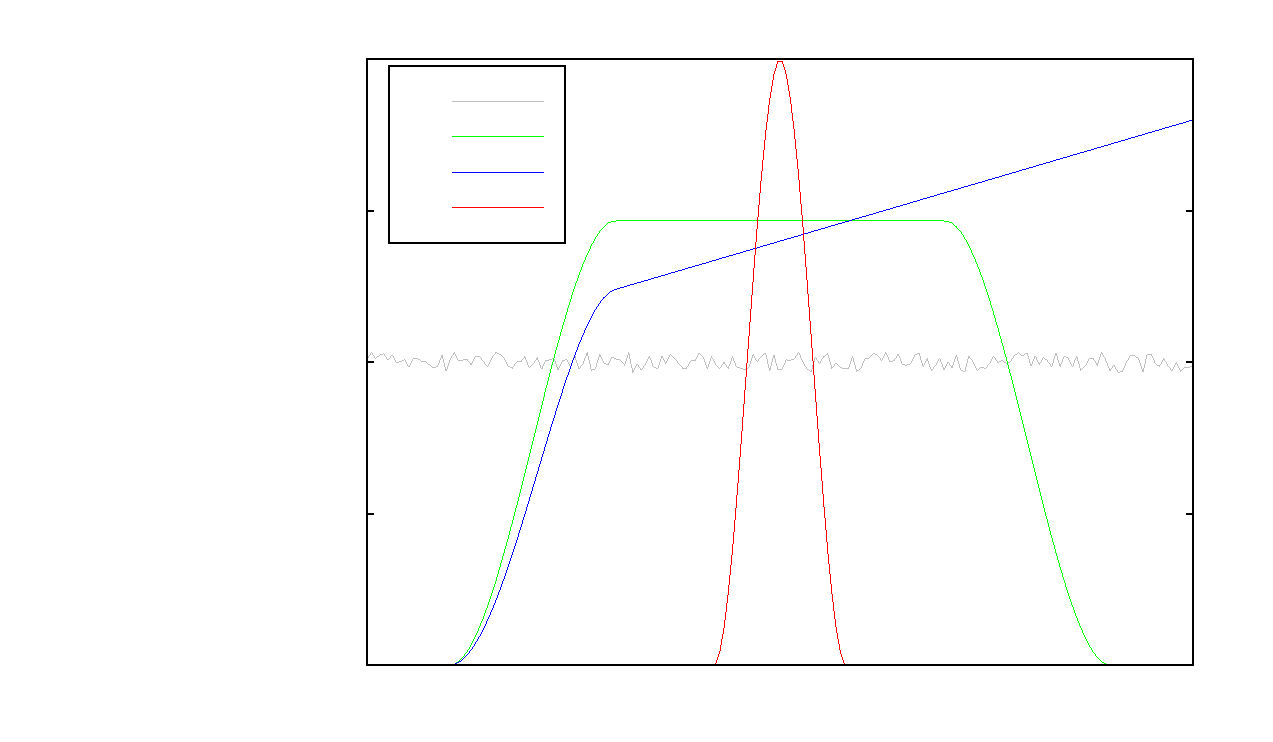
\includegraphics{fig-load-a4}}%
    \gplfronttext
  \end{picture}%
\endgroup
\else% GNUPLOT: LaTeX picture with Postscript
\begingroup
  \makeatletter
  \providecommand\color[2][]{%
    \GenericError{(gnuplot) \space\space\space\@spaces}{%
      Package color not loaded in conjunction with
      terminal option `colourtext'%
    }{See the gnuplot documentation for explanation.%
    }{Either use 'blacktext' in gnuplot or load the package
      color.sty in LaTeX.}%
    \renewcommand\color[2][]{}%
  }%
  \providecommand\includegraphics[2][]{%
    \GenericError{(gnuplot) \space\space\space\@spaces}{%
      Package graphicx or graphics not loaded%
    }{See the gnuplot documentation for explanation.%
    }{The gnuplot epslatex terminal needs graphicx.sty or graphics.sty.}%
    \renewcommand\includegraphics[2][]{}%
  }%
  \providecommand\rotatebox[2]{#2}%
  \@ifundefined{ifGPcolor}{%
    \newif\ifGPcolor
    \GPcolortrue
  }{}%
  \@ifundefined{ifGPblacktext}{%
    \newif\ifGPblacktext
    \GPblacktexttrue
  }{}%
  % define a \g@addto@macro without @ in the name:
  \let\gplgaddtomacro\g@addto@macro
  % define empty templates for all commands taking text:
  \gdef\gplbacktext{}%
  \gdef\gplfronttext{}%
  \makeatother
  \ifGPblacktext
    % no textcolor at all
    \def\colorrgb#1{}%
    \def\colorgray#1{}%
  \else
    % gray or color?
    \ifGPcolor
      \def\colorrgb#1{\color[rgb]{#1}}%
      \def\colorgray#1{\color[gray]{#1}}%
      \expandafter\def\csname LTw\endcsname{\color{white}}%
      \expandafter\def\csname LTb\endcsname{\color{black}}%
      \expandafter\def\csname LTa\endcsname{\color{black}}%
      \expandafter\def\csname LT0\endcsname{\color[rgb]{1,0,0}}%
      \expandafter\def\csname LT1\endcsname{\color[rgb]{0,1,0}}%
      \expandafter\def\csname LT2\endcsname{\color[rgb]{0,0,1}}%
      \expandafter\def\csname LT3\endcsname{\color[rgb]{1,0,1}}%
      \expandafter\def\csname LT4\endcsname{\color[rgb]{0,1,1}}%
      \expandafter\def\csname LT5\endcsname{\color[rgb]{1,1,0}}%
      \expandafter\def\csname LT6\endcsname{\color[rgb]{0,0,0}}%
      \expandafter\def\csname LT7\endcsname{\color[rgb]{1,0.3,0}}%
      \expandafter\def\csname LT8\endcsname{\color[rgb]{0.5,0.5,0.5}}%
    \else
      % gray
      \def\colorrgb#1{\color{black}}%
      \def\colorgray#1{\color[gray]{#1}}%
      \expandafter\def\csname LTw\endcsname{\color{white}}%
      \expandafter\def\csname LTb\endcsname{\color{black}}%
      \expandafter\def\csname LTa\endcsname{\color{black}}%
      \expandafter\def\csname LT0\endcsname{\color{black}}%
      \expandafter\def\csname LT1\endcsname{\color{black}}%
      \expandafter\def\csname LT2\endcsname{\color{black}}%
      \expandafter\def\csname LT3\endcsname{\color{black}}%
      \expandafter\def\csname LT4\endcsname{\color{black}}%
      \expandafter\def\csname LT5\endcsname{\color{black}}%
      \expandafter\def\csname LT6\endcsname{\color{black}}%
      \expandafter\def\csname LT7\endcsname{\color{black}}%
      \expandafter\def\csname LT8\endcsname{\color{black}}%
    \fi
  \fi
  \setlength{\unitlength}{0.0500bp}%
  \begin{picture}(5952.00,3400.00)%
    \gplgaddtomacro\gplbacktext{%
      \csname LTb\endcsname%
      \put(1488,272){\makebox(0,0)[r]{\strut{}0}}%
      \put(1488,1006){\makebox(0,0)[r]{\strut{}Низкая}}%
      \put(1488,1740){\makebox(0,0)[r]{\strut{}Средняя}}%
      \put(1488,2473){\makebox(0,0)[r]{\strut{}Высокая}}%
      \put(1488,3207){\makebox(0,0)[r]{\strut{}Экстра}}%
      \put(160,1739){\rotatebox{-270}{\makebox(0,0){\strut{}Нагрузка}}}%
      \put(3623,112){\makebox(0,0){\strut{}Время}}%
    }%
    \gplgaddtomacro\gplfronttext{%
      \csname LTb\endcsname%
      \put(1872,2984){\makebox(0,0)[r]{\strut{}1}}%
      \csname LTb\endcsname%
      \put(1872,2824){\makebox(0,0)[r]{\strut{}2}}%
      \csname LTb\endcsname%
      \put(1872,2664){\makebox(0,0)[r]{\strut{}3}}%
      \csname LTb\endcsname%
      \put(1872,2504){\makebox(0,0)[r]{\strut{}4}}%
    }%
    \gplbacktext
    \put(0,0){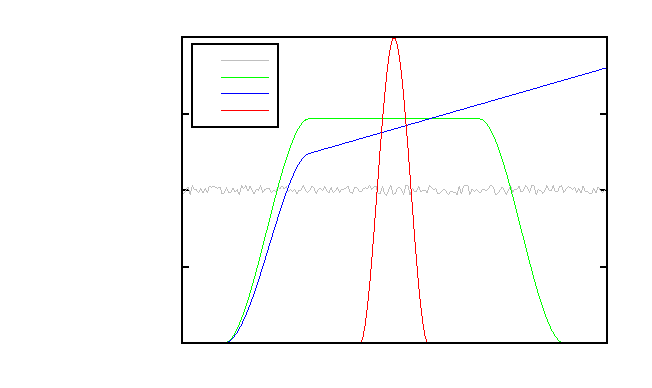
\includegraphics{fig-load}}%
    \gplfronttext
  \end{picture}%
\endgroup
\vspace{-0.25ex}\fi
			\caption{%
				Различные режимы тестирования производительности:
				\textbf{\color{gray}1} — нагрузочное тестирование \engterm{load testing};
				\textbf{\color{green}2} — стресс-тестирование \engterm{stress testing};
				\textbf{\color{blue}3} — тестирование выносливости \engterm{soak testing};
				\textbf{\color{red}4} — импульсное тестирование \engterm{spike testing}.}
		\end{figure}
	}

	\subsection{Пользовательское тестирование}

	\frame{
		\frametitle{Пользовательское тестирование}

		\begin{Definition}
			\textbf{Пользовательское тестирование} \engterm{user testing} — оценка выполнения требований к~программной системе
			с~точки зрения конечных пользователей или заказчика.
		\end{Definition}

		\vspace{1ex}
		\textbf{Виды пользовательского тестирования:}
		\begin{itemize}
			\item
			Альфа-тестирование — тестирование системы в содействии с командой разработки в~контролируемой среде.

			\textbf{Цели:} разработка реалистичных тестов; конкретизация требований.

			\item
			Бета-тестирование — тестирование промежуточного выпуска ПО, доступного для~определенного контингента пользователей.

			\textbf{Цели:} определение работоспособности в различных условиях; продвижение ПО.

			\item
			Приемочное тестирование \engterm{acceptance testing} — проверка системы заказчиком на~ее~готовность.

			\textbf{Цели:} оплата стоимости разработки; развертывание системы.
		\end{itemize}
	}

	\section{Заключение}

	\subsection{Выводы}

	\frame{
		\frametitle{Выводы}

		\begin{enumerate}
			\item
			Существует две основные цели тестирования — обнаружение ошибок и проверка (валидация) функциональности программного продукта.

			\vspace{0.5ex}
			\item
			Тестирование включает три фазы — тестирование во время разработки (\emph{development testing}),
			тестирование выпусков (\emph{release testing}) и пользовательское тестирование (\emph{user testing}).

			\vspace{0.5ex}
			\item
			В классических моделях жизненного цикла тестирование следует за конструированием ПО;
			более современный подход состоит в опережающем написании тестов (TDD).

			\vspace{0.5ex}
			\item
			Автоматизированные системы тестирования (напр., xUnit) многократно повышают эффективность тестирования вносимых в ПО изменений.
		\end{enumerate}
	}

	\subsection{Материалы}

	\frame{
		\frametitle{Материалы}

		\begin{thebibliography}{9}
			\bibitem[1]{1}
			Sommerville, Ian
			\newblock Software Engineering.
			\newblock {\footnotesize Pearson, 2011. — 790 p.}

			\bibitem[2]{2}
			Лавріщева К.\,М.
			\newblock Програмна інженерія (підручник).
			\newblock {\footnotesize К., 2008. — 319 с.}
		\end{thebibliography}
	}

	\frame{
		\frametitle{}

		\begin{center}
			\Huge Спасибо за внимание!
		\end{center}
	}
\end{document}
